% Gemini theme
% https://github.com/anishathalye/gemini
%
% We try to keep this Overleaf template in sync with the canonical source on
% GitHub, but it's recommended that you obtain the template directly from
% GitHub to ensure that you are using the latest version.

\documentclass[final, 20pt]{beamer}

% ====================
% Packages
% ====================

\usepackage[T1]{fontenc}
\usepackage{lmodern}
% \usepackage[size=custom,width=120,height=72,scale=1.0]{beamerposter}
\usepackage[size=a1,scale=1.3]{beamerposter}
\usetheme{gemini}
\usecolortheme{gemini}
\usepackage{graphicx}
\graphicspath{images}
\usepackage{booktabs}
\usepackage{tikz}
\usepackage{pgfplots}
\usepackage{lipsum}
% ====================
% Lengths
% ====================

% If you have N columns, choose \sepwidth and \colwidth such that
% (N+1)*\sepwidth + N*\colwidth = \paperwidth
\newlength{\sepwidth}
\newlength{\colwidth}
\setlength{\sepwidth}{0.025\paperwidth}
\setlength{\colwidth}{0.3\paperwidth}

\newcommand{\separatorcolumn}{\begin{column}{\sepwidth}\end{column}}

% ====================
% Title
% ====================

\title{Fiducial Autonomous Landing with a DJI Spark and April Tags}

\author{Joshua Springer}

\institute[shortinst]{Reykjavík University}

% ====================
% Body
% ====================

\begin{document}

\begin{frame}[t]
\begin{columns}[t]
\separatorcolumn

\begin{column}{\colwidth}

  \begin{alertblock}{Problem Description}

    The goal of this project is to land a drone autonomously and accurately on a safe landing pad.
    Our contribution to the previous work is to also leverage the gimbal-mounted camera for tracking,
    and to provide a new family of embeddable and computationally inexpensive April Tag markers.

    Landing is a hard part of autonomous drone flight because it is risky and requires high precision.
    GPS alone does not provide a sufficiently accurate position estimate for landing,
    so we have to use other means.
    Fiducial markers can allow a drone to recognize a landing pad cheaply and relatively reliably.
    Previous methods have used a fixed, downward facing camera to identify fiducial markers on a landing pad,
    with the disadvantage that they can easily lose track of it.
    This project presents a method of autonomous fiducial landing with a gimbal-mounted camera that can track the marker,
    giving the advantage that the drone doesn't lose sight of the landing pad easily,
    but with the disadvantage that the drone must accurately detect not only the position,
    but also the orientation of the landing pad.
    The orientation is particularly hard to accurately detect because of the camera's limited pixel resolution and distortions.

  \end{alertblock}

  \begin{block}{Methods}

    \heading{Flight Control Software}

    DJI provides proprietary flight control software on its drones,
    and we interact with it through a \textbf{Mobile SDK} interface
    to give high level commands (i.e.~``go left,'' ``go forward,'' ``land,'' etc).
    With no input the flight control software keeps the drone almost perfectly still.

    \heading{Localization \& Tracking with April Tag 48h12}

    We use a fiducial marker system called April Tag to locate the landing pad in real time using the drone's onboard camera.
    The system can determine a marker's \textbf{pose} (position + orientation) in space with respect to the camera.
    Using coordinate system transforms, we can rotate the pose by the inverse of the pitch and roll components of the orientation,
    and this gives the position of the drone in the coordinate frame of landing pad (ignoring yaw).
    From this, we can determine which direction the drone must move in order to approach the landing pad.
    The drone uses the yaw of the landing pad to align itself once it is sufficiently close in order to make the landing pad easier to track.
    The April Tag system also determines the $(x,y)$ pixel positions of the centers of any detected markers,
    which are normalized in the interval $[-1,1]$.
    This makes it easy to track the landing pad (i.e.~keep its $(x,y)$ pixel positions near $(0,0)$)
    so that it is cenetered in the camera frame and not lost during approach.

  \end{block}

\end{column}

\separatorcolumn

\begin{column}{\colwidth}

  \begin{block}{Marker System}

    \begin{figure}
      \centering
      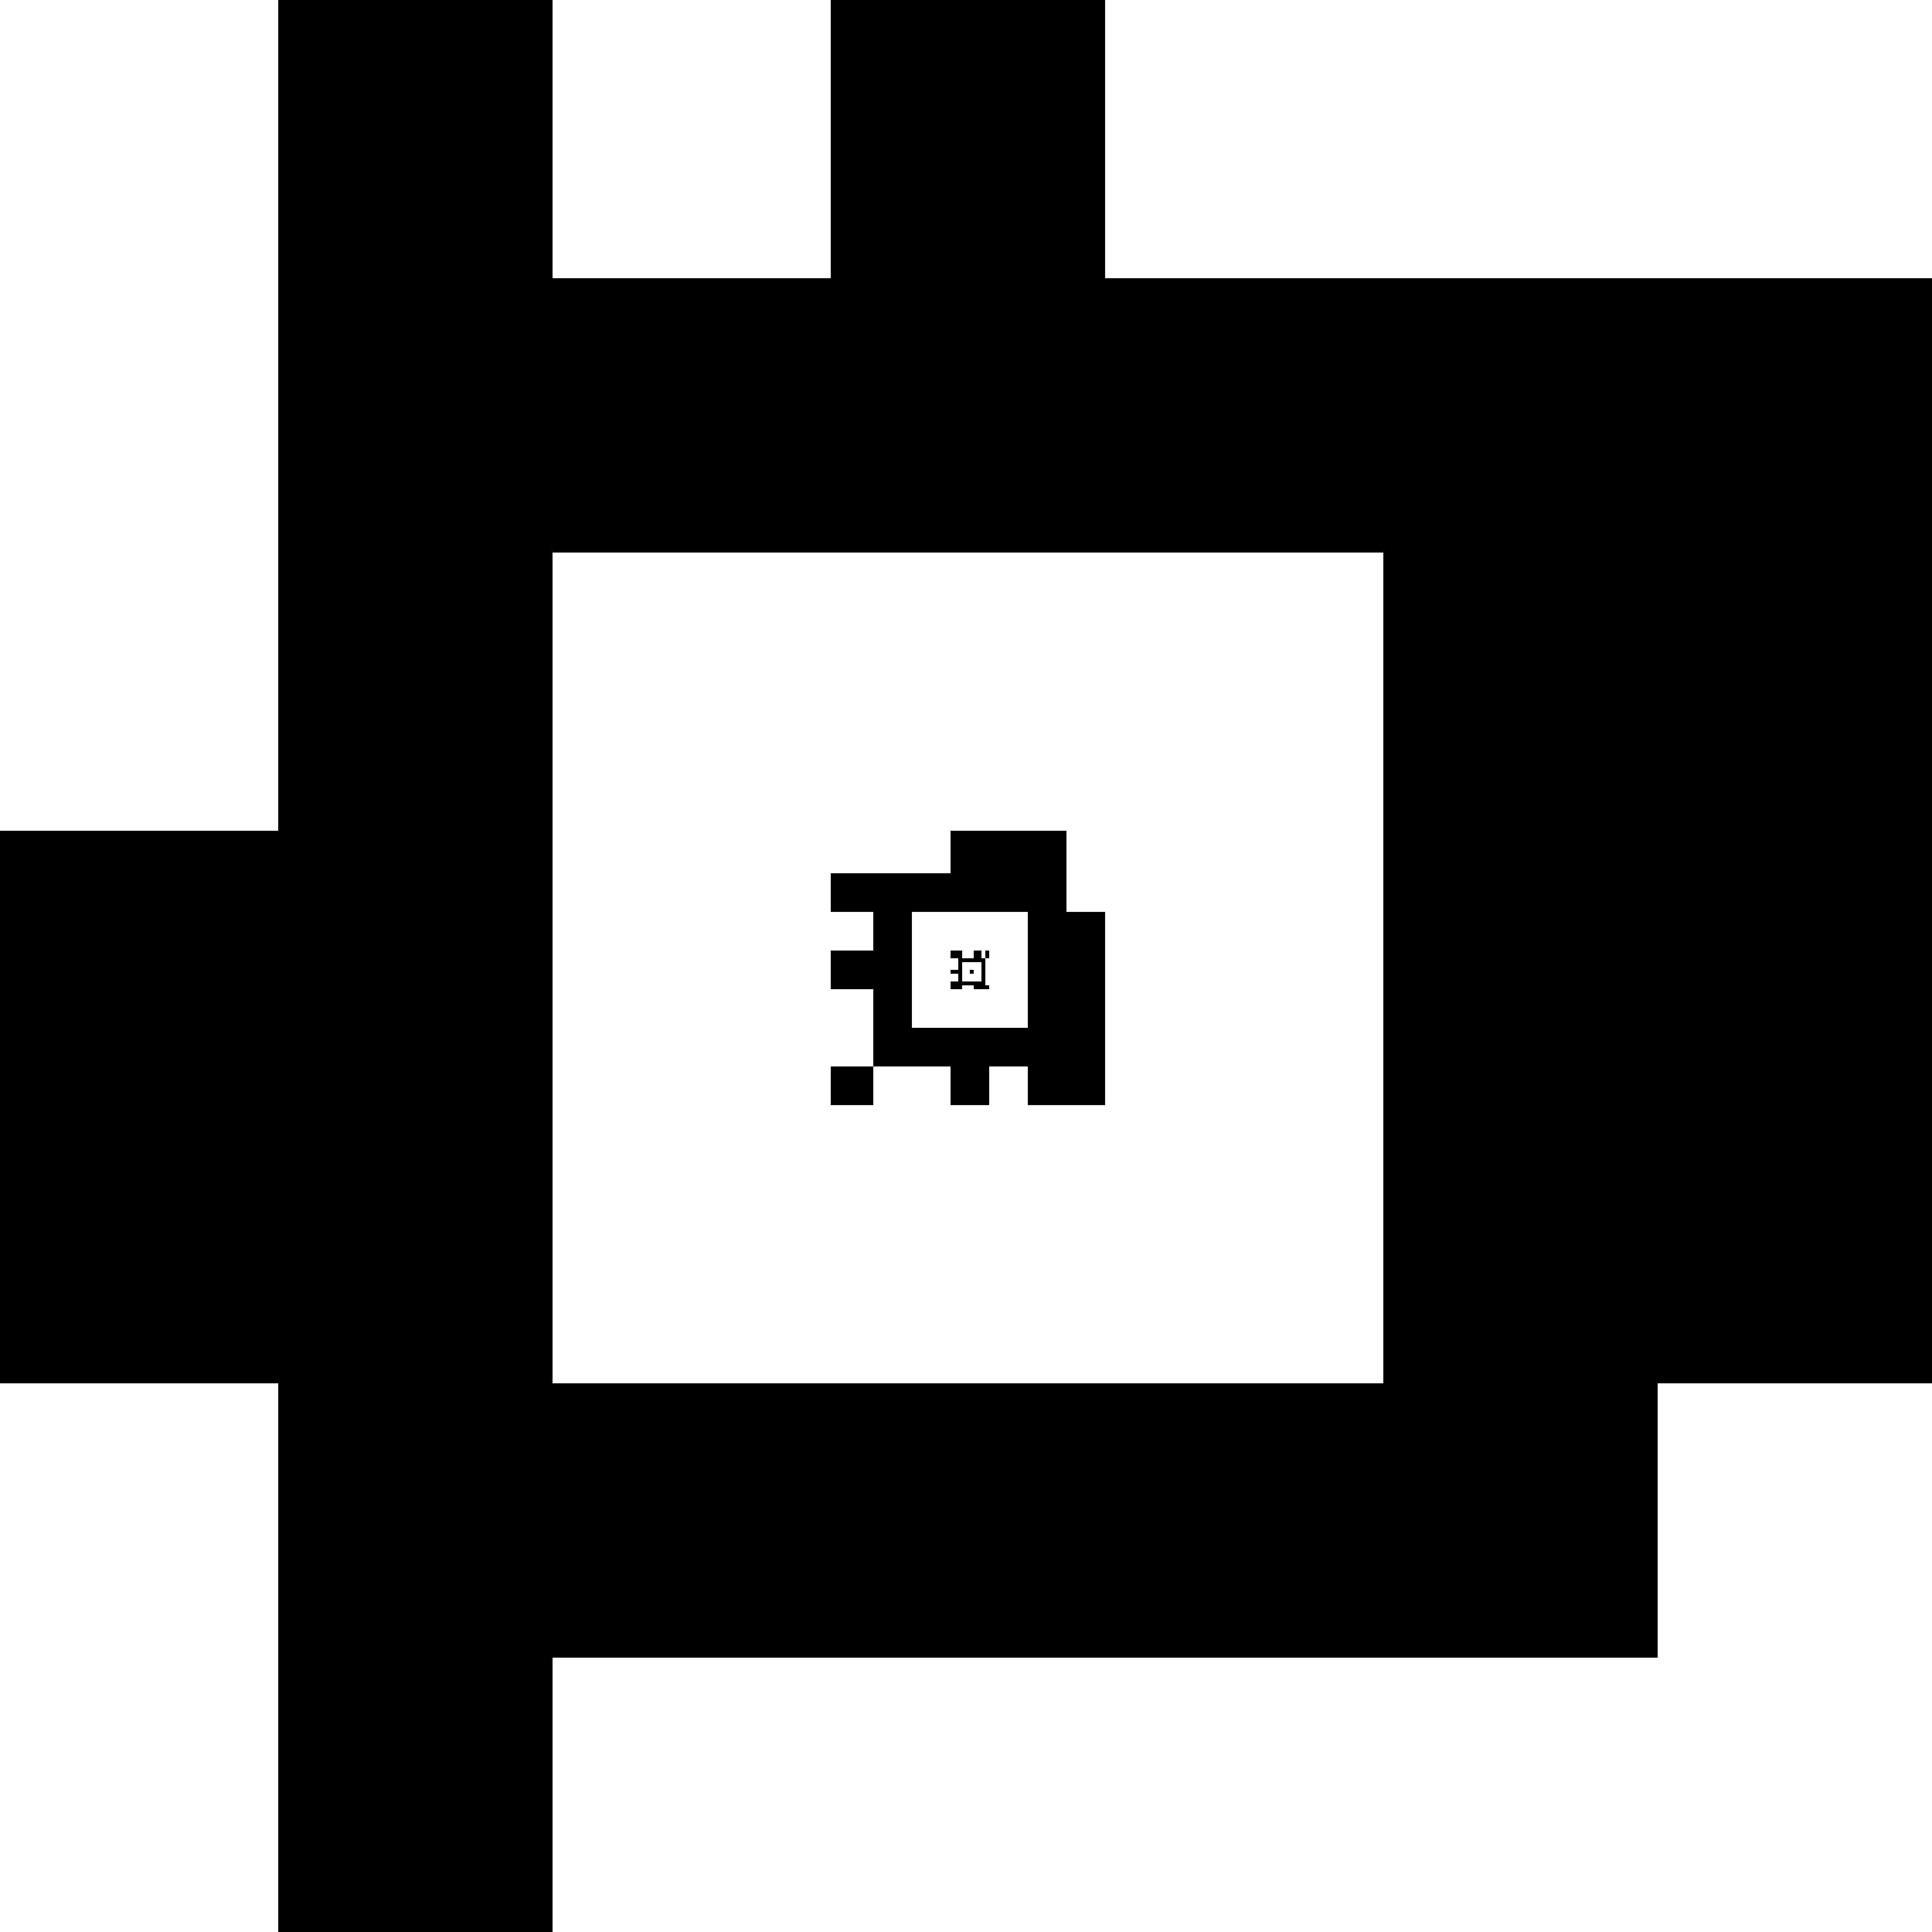
\includegraphics[width=5cm]{images/tagCustom24h10_00002_00001_00000}
      \caption{The landing pad with 3 embedded April Tags of the 24h10 family.}
    \end{figure}

  \end{block}

  \begin{alertblock}{System Design \& Equipment}

    \lipsum[10]

    \begin{figure}
      \centering
      
\includegraphics[width=\linewidth]{images/spark_architecture.drawio}
      \caption{System data flow.}
    \end{figure}

    \lipsum[15]

  \end{alertblock}

%  \begin{block}{Equipment}
%
%    \begin{itemize}
%      \item \textbf{Sed consequat} id ante vel efficitur. Praesent congue massa
%        sed est scelerisque, elementum mollis augue iaculis.
%        \begin{itemize}
%          \item In sed est finibus, vulputate
%            nunc gravida, pulvinar lorem. In maximus nunc dolor, sed auctor eros
%            porttitor quis.
%          \item Fusce ornare dignissim nisi. Nam sit amet risus vel lacus
%            tempor tincidunt eu a arcu.
%          \item Donec rhoncus vestibulum erat, quis aliquam leo
%            gravida egestas.
%        \end{itemize}
%      \item \textbf{Sed luctus, elit sit amet} dictum maximus, diam dolor
%        faucibus purus, sed lobortis justo erat id turpis.
%      \item \textbf{Pellentesque facilisis dolor in leo} bibendum congue.
%        Maecenas congue finibus justo, vitae eleifend urna facilisis at.
%    \end{itemize}
%
%  \end{block}

\end{column}

\separatorcolumn

\begin{column}{\colwidth}

  \begin{alertblock}{Results}

    Nullam non est elit. In eu ornare justo. Maecenas porttitor sodales lacus,
    ut cursus augue sodales ac.

    $$
    \int_{-\infty}^{\infty} e^{-x^2}\,dx = \sqrt{\pi}
    $$

    Interdum et malesuada fames $\{1, 4, 9, \ldots\}$ ac ante ipsum primis in
    faucibus. Cras eleifend dolor eu nulla suscipit suscipit. Sed lobortis non
    felis id vulputate.

    \heading{A heading inside a block}

    Praesent consectetur mi $x^2 + y^2$ metus, nec vestibulum justo viverra
    nec. Proin eget nulla pretium, egestas magna aliquam, mollis neque. Vivamus
    dictum $\mathbf{u}^\intercal\mathbf{v}$ sagittis odio, vel porta erat
    congue sed. Maecenas ut dolor quis arcu auctor porttitor.

    \heading{Another heading inside a block}

    Sed augue erat, scelerisque a purus ultricies, placerat porttitor neque.
    Donec $P(y \mid x)$ fermentum consectetur $\nabla_x P(y \mid x)$ sapien
    sagittis egestas. Duis eget leo euismod nunc viverra imperdiet nec id
    justo.

    \heading{Lipsum}
    \lipsum[50-51]

  \end{alertblock}

%  \begin{block}{Results}
%
%    Class aptent taciti sociosqu ad litora torquent per conubia nostra, per
%    inceptos himenaeos. Phasellus libero enim, gravida sed erat sit amet,
%    scelerisque congue diam. Fusce dapibus dui ut augue pulvinar iaculis.
%
%    \begin{table}
%      \centering
%      \begin{tabular}{l r r c}
%        \toprule
%        \textbf{First column} & \textbf{Second column} & \textbf{Third column} & \textbf{Fourth} \\
%        \midrule
%        Foo & 13.37 & 384,394 & \alpha \\
%        Bar & 2.17 & 1,392 & \beta \\
%        Baz & 3.14 & 83,742 & \delta \\
%        Qux & 7.59 & 974 & \gamma \\
%        \bottomrule
%      \end{tabular}
%      \caption{A table caption.}
%    \end{table}
%
%  \end{block}

  \begin{block}{References}

    \nocite{*}
    \footnotesize{\bibliographystyle{plain}\bibliography{poster}}

  \end{block}

\end{column}

\separatorcolumn
\end{columns}
\end{frame}

\end{document}
